%% img/nondeterminism/Canonicalization.tex
%% Copyright 2019 Andrea Berlingieri
%
% This work may be distributed and/or modified under the
% conditions of the LaTeX Project Public License, either version 1.3
% of this license or (at your option) any later version.
% The latest version of this license is in
%   http://www.latex-project.org/lppl.txt
% and version 1.3 or later is part of all distributions of LaTeX
% version 2005/12/01 or later.
%
% This work has the LPPL maintenance status `maintained'.
%
% The Current Maintainer of this work is Andrea Berlingieri.
%
% This work consists of all files listed in manifest.txt
\documentclass{standalone}

\usepackage{../TikzStyle}
\usepackage{../mystyle}
\usetikzlibrary{automata}

\begin{document}
    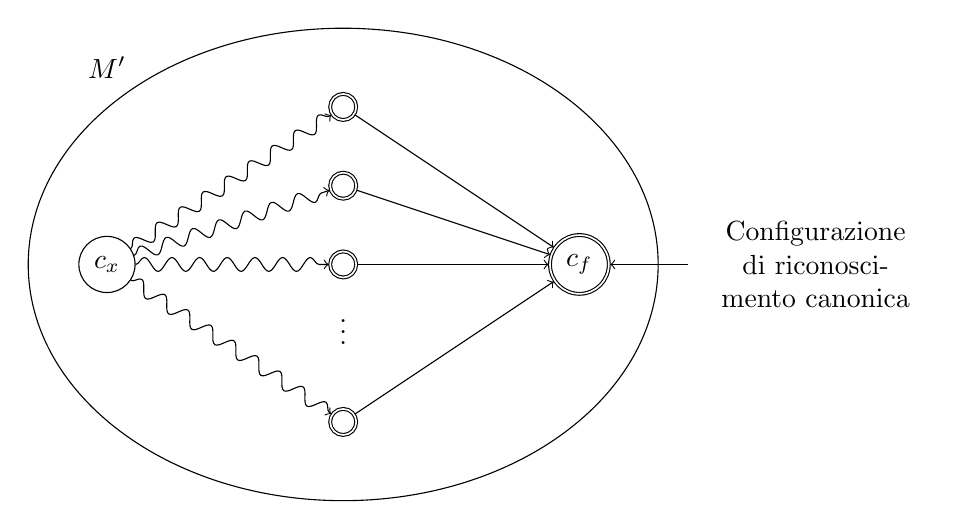
\begin{tikzpicture}
        \draw (0,0) ellipse [x radius=4cm, y radius=3cm];
        \node () at (-3,2.5) {$M'$};
        \node[state,minimum size=3mm] (initial) at (-3,0) {$c_{x}$};
        \node[state,accepting,minimum size=3mm] (c1) at (0,2) {};
        \node[state,accepting,minimum size=3mm] (c2) at (0,1) {};
        \node[state,accepting,minimum size=3mm] (c3) at (0,0) {};
        \node () at (0,-0.75) {$\vdots$};
        \node[state,accepting,minimum size=3mm] (c4) at (0,-2) {};
        \node[state,accepting,minimum size=3mm] (final) at (3,0) {$c_{f}$};
        %\node[state,accepting,minimum size=3mm] (final) at (5,-1.2) {};
        \draw[->,decorate,decoration=snake] (initial) -- (c1);
        \draw[->,decorate,decoration=snake] (initial) -- (c2);
        \draw[->,decorate,decoration=snake] (initial) -- (c3);
        \draw[->,decorate,decoration=snake] (initial) -- (c4);

        \draw[->] (c1) -- (final);
        \draw[->] (c2) -- (final);
        \draw[->] (c3) -- (final);
        \draw[->] (c4) -- (final);


        \node[text width=3cm, align=center] (descr) at (6,0) {Configurazione di riconoscimento canonica};
        \draw[<-] (final) -- (descr);
    \end{tikzpicture}
\end{document}
